\chapter{Analisi di dati numerici}
Procediamo con alcune definizioni fondamentali per l'analisi statistica dei dati.

\begin{definition} \label{vettore}
	Definiamo \textbf{vettore di dati}, un insieme di valori, potenzialmente tutti diversi.
	\[ x = (x_1, x_2, \dots, x_n) \]
\end{definition}

\begin{definition}
	Definiamo la \textbf{media empirica} o il \textbf{valore medio} come la media aritmetica dei
	valori in un certo vettore di dati.
	\[ \overline{x} = \frac{x_1 + x_2 + \dots + x_n}{n} \]
\end{definition}

\section{Varianza}

\begin{definition}
	Sia $x$ un vettore di dati, definiamo la \textbf{varianza campionaria} come
	\[ \Var(x) = \frac{1}{n - 1} \cdot \sum_{i=1}^n (x_i - \overline{x})^2 \]
	La varianza campionaria si applica meglio su campioni di dati.
\end{definition}

\begin{definition}
	Sia $x$ un vettore di dati, definiamo la \textbf{varianza empirica} come
	\[ \Var_e(x) = \frac{1}{n} \sum_{i=1}^n (x_i - \overline{x})^2 \]
	La varianza empirica si applica meglio su intere popolazioni di dati.
\end{definition}

Definiamo anche un'uguaglianza di base che, per il momento non andremo a spiegare, ma che in
seguito ci tornerà utile:
\[ \sum_{i=1}^n (x_i - \overline{x})^2 = \sum_{i=1}^n x_i^2 - n \overline{x}^2 \]
\begin{proof}
	Sviluppando il quadrato possiamo facilmente convincerci che l'uguaglianza sia vera:
	\begin{align*}
		\sum_{i=1}^n (x_i - \overline{x})^2 =                                     \\
		\sum_{i=1}^n (x_i^2 - 2 x_i \overline{x} + \overline{x}^2) =              \\
		\sum_{i=1}^n x_i^2 - 2 \overline{x} \sum_{i=1}^n x_i + n \overline{x}^2 = \\
		\sum_{i=1}^n x_i^2 - 2 n \overline{x}^2 + n \overline{x}^2 =              \\
		\sum_{i=1}^n x_i^2 - n \overline{x}^2
	\end{align*}
\end{proof}

\begin{definition}
	Definiamo lo \textbf{scarto quadratico medio} come la radice quadrata della varianza
	campionaria:
	\[ \sigma (x) = \sqrt{\Var (x)} \]
\end{definition}

\begin{definition}
	Definiamo la \textbf{deviazione standard} come la radice quadrata della varianza empirica:
	\[ \sigma_e (x) = \sqrt{\Var_e (x)} \]
\end{definition}

\section{Concentrazione dei dati}

\begin{definition}
	Definiamo ora una \textbf{regola empirica sulla concentrazione dei dati}: supponendo che
	l'istogramma sia normale abbiamo che
	\begin{itemize}
		\item Circa il 68\% dei dati appartiene a
		      \[ [ \overline{x} - \sigma(x),\; \overline{x} + \sigma(x) ] \]
		\item Circa il 95\% dei dati appartiene a
		      \[ [ \overline{x} - 2 \sigma(x),\; \overline{x} + 2 \sigma(x) ] \]
		\item Circa il 99.7\% dei dati appartiene a
		      \[ [ \overline{x} - 3 \sigma(x),\; \overline{x} + 3 \sigma(x) ] \]
	\end{itemize}
	Questi intervalli si allargano tanto più velocemente quanto più grande è lo scarto quadratico
	medio (o la varianza).
\end{definition}

\begin{definition}
	Definiamo la \textbf{funzione di ripartizione empirica} come
	\[ F_e(t) = \frac{\{ x_i : x_i \leq t \}}{n} \]
	Quello che la funzione fa in pratica è prendere la percentuale dei dati che vengono prima di
	$t$.
\end{definition}

Supponendo di avere un certo insieme di dati, il procedimento per calcolare la funzione appena
definita è il seguente:
\begin{enumerate}
	\item Disporre i dati in ordine crescente:
	\item Si parte da 0 e si compie un \emph{salto} di ampiezza $1 / n$ sull'asse $y$ in
	      corrispondenza di uno dei dati. Nel caso in cui ci siano $m$ dati coincidenti, il salto
	      in quel punto sarà di $m / n$.
\end{enumerate}

\subsection{Percentili e quantili}

\begin{definition}
	Sia $k$ un numero (non necessariamente intero) compreso tra 0 e 100, diciamo che l'intero $t$
	è il $k$-esimo
	\textbf{percentile}, se
	\begin{itemize}
		\item Almeno $k / 100$ dati sono inferiori o uguali di $t$.
		\item Almeno $1 - (k / 100)$ dati sono superiori o uguali a $t$.
	\end{itemize}
	Intuitivamente si tratta del più piccolo numero che supera il $k \%$ dei dati.
\end{definition}

\begin{definition}
	Sia $\beta$ un numero compreso tra 0 e 1, diciamo che $t$ è quel valore dell'insieme tale che
	almeno $\beta \cdot n$ dati sono inferiori o uguali a $t$, e almeno $(1-\beta) \cdot n$ dati
	sono superiori a $t$.
\end{definition}

\begin{definition}
	Definiamo anche i \textbf{quartili} ($i/4$-quantili) come segue:
	\begin{itemize}
		\item Il \textbf{primo quartile} equivale allo $0.25$-quantile.
		\item La \textbf{mediana} o \textbf{secondo quartile} equivale allo $0.50$-quantile.
		\item Il \textbf{terzo quartile} equivale allo $0.75$-quantile.
	\end{itemize}
\end{definition}

\section{Dati multipli}
\subsection{Covarianza}
La \textbf{covarianza} è la misura di \emph{quanto varia} un insieme.

\begin{definition}
	Siano $x$  e $y$ due vettori di dati, definiamo la \textbf{covarianza campionaria} come
	\[ \Cov(x, y) = \frac{1}{n - 1} \sum_{i=1}^n (x_i - \overline{x}) (y_i - \overline{y}) \]
\end{definition}

\begin{definition}
	Siano $x$  e $y$ due vettori di dati, definiamo la \textbf{covarianza empirica} come
	\[
		\Cov_e(x, y) = \frac{1}{n} \sum_{i=1}^n (x_i - \overline{x}) (y_i - \overline{y}) =
		\frac{1}{n} \left( \sum_{i=1}^n x_i \cdot y_i \right) - \overline{x} \cdot \overline{y}
	\]
\end{definition}

\begin{definition}
	Supponiamo $\sigma (x) \neq 0$ e $\sigma (y) \neq 0$, allora chiamiamo
	\textbf{coefficiente di correlazione} tra $x$ e $y$ il numero
	\[
		r(x, y) = \frac{\Cov (x, y)}{\sigma (x) \cdot \sigma (y)} =
		\frac{\sum_{i=1}^n (x_i - \overline{x})(y_i - \overline{y})}
		{\sqrt{\sum_{i=1}^n (x_i - \overline{x})^2} \cdot
			\sqrt{\sum_{i=1}^n (y_i - \overline{y})^2}}
	\]
	Sia che si scelga la covarianza campionaria sia che si scelga quella empirica il risultato
	non cambia.
\end{definition}

\begin{definition}
	La \textbf{disuguaglianza di Schwartz} è definita come segue
	\[
		\sum_{i=1}^n |(x_i - \overline{x}) (y_i - \overline{y})| \leq
		\sqrt{\sum_{i=1}^n (x_i - \overline{x})^2} \cdot \sqrt{\sum_{i=1}^n (y_i - \overline{y})^2}
	\]
	e di conseguenza vale \[ |r(x, y)| \leq 1 \]
\end{definition}

Intuitivamente il \emph{coefficiente di correlazione} misura il \emph{legame lineare} che c'è tra
i dati $x$ e $y$ ma per comprendere meglio il concetto dobbiamo introdurre la
\textbf{retta di regressione}.

\subsection{Rette di regressione}
Per calcolare una \textbf{retta di regressione} facciamo ovviamente riferimento all'equazione
generica di una retta
\[ y = a x + b \]
Per calcolare la retta di regressione su un certo insieme di dati dobbiamo trovare $a$ e $b$ tali
che la distanza fra la retta e i punti sia minima.

In altre parole stiamo cercando di \emph{approssimare} al meglio i dati un insieme di dati
calcolando la retta che lo fa con il minor errore di approssimazione possibile.

Di seguito troviamo l'equazione che ci fornisce l'\textbf{errore quadratico medio} di una retta di
regressione
\[ Q(a, b) = \sum_{i=1}^n (y_i - (a x_i + b))^2 \]
Come possiamo vedere, l'\emph{errore quadratico medio}, si calcola facendo la differenza tra
$y_i$, ossia uno dei dati nel vettore $y$ e $a x_i + b$, ossia il valore della retta con $x_i$
come valore sulle ascisse.

Dato che l'\emph{errore quadratico medio} della retta è la somma degli errori di approssimazione
su tutti i punti della retta, e questi possono essere anche negativi, non si fa una pura di tutti
gli errori, ma del loro quadrato, di modo da averli tutti positivi e di modo da poter minimizzare
meglio la funzione.

\begin{theorem}
	Il minimo, al variare di $(a, b) \in \mathbb{R}^2$, della quantità
	\[ \sum_{i=1}^n (y_i - (a x_i + b))^2 \]
	si ottiene calcolando i coefficienti $a^*$ e $b^*$ come segue
	\[ a^* = \frac{\Cov(x, y)}{\Var(x)} \quad \wedge \quad b^* = \overline{y} - a^* \overline{x} \]
	e vale l'uguaglianza
	\[
		\min_{a, b \in \mathbb{R}^2} \sum_{i=1}^n (y_i - (a x_i + b))^2 =
		(1 - r(x, y)^2) \cdot \sum_{i=1}^n (y_i - \overline{y})^2
	\]
	La retta $y = a^* x + b^*$ è chiamata \textbf{retta di regressione}.
	\begin{proof}
		Quel che vogliamo fare è minimizzare la funzione
		\[ Q(a, b) = \sum_{i=1}^n (y_i - (a x_i + b))^2 \]
		al variare di $a$ e $b$. Come è possibile notare dal calcolo del limite
		\[ \lim_{|a|, |b| \to +\infty} Q(a, b) = +\infty \]
		si tratta di una funzione a valori positivi che tende a $+\infty$ quando $a$ e $b$
		tendono a
		$\pm\infty$.

		Per trovare il minimo di una funzione a due variabili si annullano le derivate parziali
		rispetto a $a$ e $b$
		\[ \frac{\partial Q}{\partial a} = 0 \quad \frac{\partial Q}{\partial b} = 0 \]
		Dobbiamo quindi andare a risolvere un sistema a due equazioni di questo tipo
		\[
			\begin{cases}
				\sum_{i=1}^n x_i y_i - a \sum_{i=1}^n x_i^2 - b \sum_{i=1}^n x_i & = 0 \\
				\sum_{i=1}^n y_i - a \sum_{i=1}^n x_i - n b                      & = 0
			\end{cases}
		\]
		Dividendo per $n$ entrambe le equazioni si arriva a
		\[
			\begin{cases}
				\frac{1}{n} \sum_{i=1}^n x_i y_i - \frac{a}{n} \sum_{i=1}^n x_i^2 +
				b \overline{x}                    & = 0 \\
				\overline{y} - a \overline{x} - b & = 0
			\end{cases}
		\]
		Risolvendo il sistema si ricavano $a$ e $b$ come segue
		\[
			\begin{cases}
				b = & \overline{y} - a \overline{x}            \\
				a = & \frac{\frac{1}{n} \sum_{i=1}^n x_i y_i -
					\overline{x} \cdot \overline{y}}
				{\frac{1}{n} \sum_{i=1}^n x_i^2 - \overline{x}^2} =
				\frac{\Cov_e(x, y)}{\Var_e(x)}
			\end{cases}
		\]
		Otteniamo così $a^*$ e $b^*$ e se proviamo a calcolare $Q(a^*, b^*)$ si ricava che
		\[ Q(a^*, b^*) = \sum_{i=1}^n (y_i - \overline{y})^2 (1 - r(x, y)^2) \]
	\end{proof}
\end{theorem}

\begin{observation}
	Il \textbf{valore assoluto} del coefficiente di correlazione ci fornisce quindi delle
	informazioni interessanti sui dati:
	\begin{itemize}
		\item $|r(x, y)| = 1$ se e solo se i dati sono tutti sulla stessa retta.
		\item $|r(x, y)| \approx 1$ se i dati sono molto allineati.
		\item $|r(x, y)| \approx 0$ se i dati sono dispersi.
	\end{itemize}
	Possiamo anche notare che il \textbf{segno} del coefficiente di correlazione ci fornisce
	un'altra informazione interessante:
	\begin{itemize}
		\item Se $r(x, y) < 0$ allora la retta decresce al crescere di $x$.
		\item Se $r(x, y) > 0$ allora la retta cresce al crescere di $x$.
	\end{itemize}
\end{observation}

\begin{example}
	Proviamo ora a calcolare la retta di regressione su un insieme di dati contenuto. Supponiamo
	di avere 5 maschi e 5 femmine della stessa età e, per ognuno di essi, sappiamo altezza e peso.
	\begin{center}
		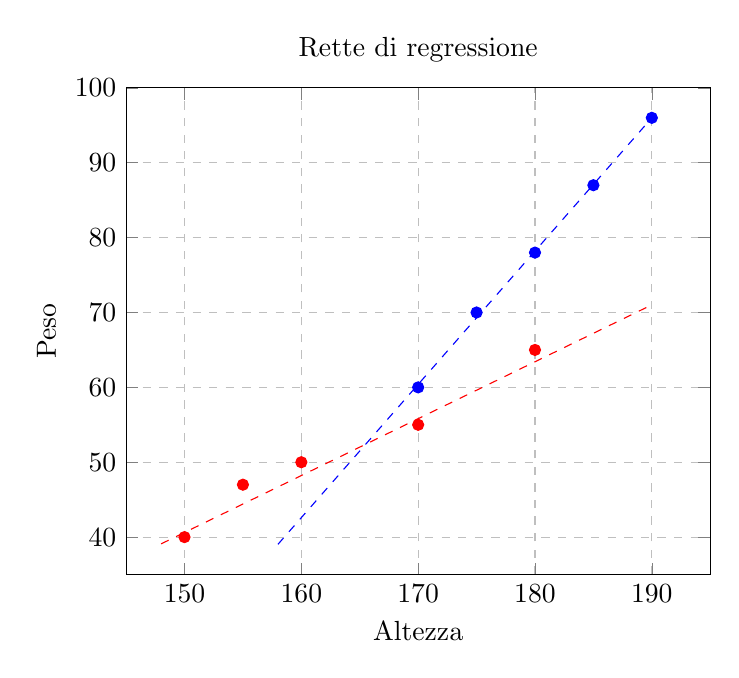
\begin{tikzpicture}
			\begin{axis}[
					title={Rette di regressione},
					xmin=145, xmax=195,
					ymin=35, ymax=100,
					xlabel={Altezza},
					ylabel={Peso},
					width=9cm,
					grid=both,
					grid style=dashed,
					legend pos=north west
				]
				\addplot [blue, only marks] coordinates{
						(170, 60)
						(175, 70)
						(180, 78)
						(185, 87)
						(190, 96)
					};

				\addplot [blue, domain=158:190, dashed] {1.78 * x - 242.2};

				\addplot [red, only marks] coordinates{
						(150, 40)
						(155, 47)
						(160, 50)
						(170, 55)
						(180, 65)
					};

				\addplot [red, domain=148:190, dashed] {0.76 * x - 73.38};
			\end{axis}
		\end{tikzpicture}
	\end{center}
	Come possiamo notare abbiamo due rette che passano molto vicine ai dati, ma hanno coefficiente
	angolare differente.

	Sia per maschi che per femmine possiamo dire che, più un ragazzo è alto, più è pesante. Il
	fatto che però le due rette crescano in modo differente ci dice che le ragazze hanno un
	rapporto peso-altezza più basso dei maschi.
\end{example}
